% v2-acmlarge-sample.tex, dated March 6 2012
% This is a sample file for ACM large trim journals
%
% Compilation using 'acmlarge.cls' - version 1.3, Aptara Inc.
% (c) 2011 Association for Computing Machinery (ACM)
%
% Questions/Suggestions/Feedback should be addressed to => "acmtexsupport@aptaracorp.com".
% Users can also go through the FAQs available on the journal's submission webpage.
%
% Steps to compile: latex, bibtex, latex latex
%
\documentclass[prodmode,acmtap]{acmlarge}

% Metadata Information
\acmVolume{2}
\acmNumber{3}
\acmArticle{1}
\articleSeq{1}
\acmYear{2010}
\acmMonth{5}

% Package to generate and customize Algorithm as per ACM style
\usepackage[ruled]{algorithm2e}
\usepackage{comment}
\usepackage{todonotes}
\usepackage[square,sort]{natbib}
\usepackage{graphics}
\usepackage{caption}
\usepackage{commath}
\usepackage{amsfonts}
\usepackage{graphicx}
\SetAlFnt{\algofont}
\SetAlCapFnt{\algofont}
\SetAlCapNameFnt{\algofont}
\SetAlCapHSkip{0pt}
\IncMargin{-\parindent}
\renewcommand{\algorithmcfname}{ALGORITHM}

% Page heads
\markboth{A. Sperlea and D. Arneson}{Demonstrating that Epigenomic Modifications are Cell-Type Specific Through Clustering and Identifying Biologically Relevant Domains}

% Title portion
\title{Demonstrating that Epigenomic Modifications are Cell-Type Specific Through Clustering and Identifying Biologically Relevant Domains}
\author{ADRIANA SPERLEA and DOUGLAS ARNESON \affil{University of California Los Angeles}}
% NOTE! Affiliations placed here should be for the institution where the
%       BULK of the research was done. If the author has gone to a new
%       institution, before publication, the (above) affiliation should NOT be changed.
%       The authors 'current' address may be given in the "Author's addresses:" block (below).
%       So for example, Mr. Fogarty, the bulk of the research was done at UIUC, and he is
%       currently affiliated with NASA.

\begin{abstract}
Need to write Abstract Together
\end{abstract}

\terms{Epigenomics}
\keywords{Chromatin modifications, PCA, Clustering, F-Score, Purity}

\acmformat{Adriana Sperlea and Douglas Arneson. 2015. Demonstrating that Epigenomic Modifications are Cell-Type Specific Through Clustering and Identifying Biologically Relevant Domains.}
% At a minimum you need to supply the author names, year and a title.
% IMPORTANT:
% Full first names whenever they are known, surname last, followed by a period.
% In the case of two authors, 'and' is placed between them.
% In the case of three or more authors, the serial comma is used, that is, all author names
% except the last one but including the penultimate author's name are followed by a comma,
% and then 'and' is placed before the final author's name.
% If only first and middle initials are known, then each initial
% is followed by a period and they are separated by a space.
% The remaining information (journal title, volume, article number, date, etc.) is 'auto-generated'.

\begin{document}

\begin{bottomstuff}
STATSM254 Final Report
\end{bottomstuff}


\maketitle

% Head 1
\section{Introduction}

The recent availability of epigenomic data sets such as histone modifications or DNA methylation, coupled with the growing popularity of applying machine learning techniques to genomic data have enabled the computational imputation of genome-wide cross-sample epigenetic marks. In the paper by \citealp{Ernst15}, the authors developed a method called ChromImpute that accurately predicts a variety of epigenomic data in 127 human cell lines originating from a diverse set of tissues.
Previous work has shown that although histone modifications are not cell type specific at promoter and transcription factor binding sites, they show a high level of cell type specificity at enhancer sites, which they are strongly associated with (\citealp{Hein09}). Thus, it is expected that similar cell types will exhibit similar epigenetic marks. Here, we show that the imputed data from \citealp{Ernst15} preserves the cell-type specific aspect of chromatin modifications by running a principal component analysis (PCA) on the dataset from their paper, and then clustering the resulting distribution of cell lines. Certain histone modifications were more cell type specific and thus more accurately assigned similar types to the same cluster.
We attempted to gain insight into the biological function of the genomic regions that proved to be most important to the PCA in a certain chromatin modification, and particularly to those that were present across marks by cross-checking these regions with known annotations of the human genome. These regions fell predominantly in non-coding regions, but exhibited a potential association with enhancer sites.

% Head 2
\section{Principal Component Analysis}

The imputed data from \citealp{Ernst15}. consists of 9 different chromatin modifications in 127 different cell-types, with a corresponding p-value for each bin of 500 base pairs in the genome indicating the likelihood of having that particular mark at that location. In order for our problem to remain computationally tractable we restricted our analysis to chromosome 21, though data is available for the entire human genome. For each of these 9 chromatin modifications we normalized the data such that the p-values for every location in the genome have mean 0 and variance 1 (Figure~\ref{fig:figure1}). 

\begin{figure}[tp]
\centering
\begin{minipage}{.5\textwidth}
	\centering
	\scalebox{.45}{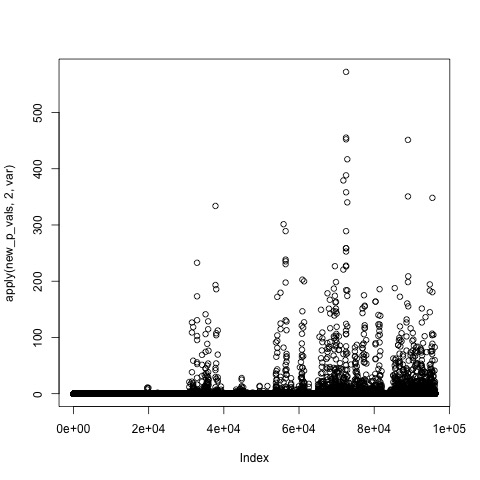
\includegraphics{varPlot1}}
\end{minipage}%
\begin{minipage}{.5\textwidth}
	\centering
	\scalebox{.45}{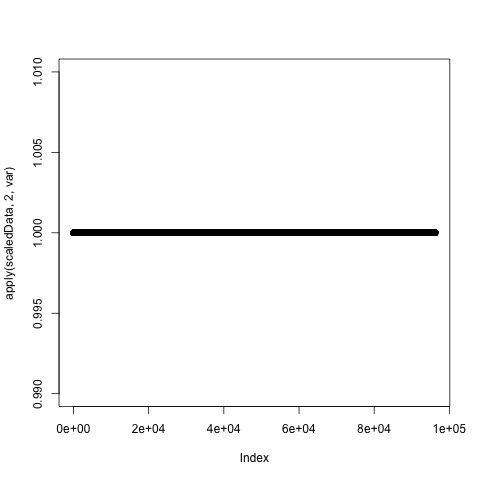
\includegraphics{varPlot2}}	
\end{minipage}	
\captionof{figure}{H3Kme27ac variance of p-values across chromosome 21 before and after normalization. After normalization, the p-values show an uniform distribution. See Supplementary Materials for the variance of the other chromatin modifications before and after normalization.}
\label{fig:figure1}
\end{figure}

After normalization, we ran a principal component analysis on each of the 9 chromatin modifications. Our results show that upwards of 30 principal components were necessary to explain 85\% of the variance which is a common threshold used in the literature, but by analyzing the scree plots of the variance of each component we were able to restrict the number of important components further. We used the broken-stick method \citealp{Cang07} to quantify the point in the turn in the scree graph where retaining an additional principal component would be of no benefit (Figure~\ref{fig:figure2}). The number of principal components retained in each epigenetic mark are available in Table~\ref{table:tab1}.

% Table
\begin{table}[h]
\tbl{Number of principal components retained}{
\resizebox{\textwidth}{!}
{%
\begin{tabular}{|l|l|l|l|l|l|l|l|l|l|}
\hline
Epigenetic Mark                         & DNase & H3K4me1 & H3K4me3 & H3K9ac & H3K9me3 & H3K27ac & H3K27me3 & H3K36me3 & RNAseq \\ \hline
Number of principal components retained & 3     & 5       & 3       & 4      & 5       & 4       & 3        & 5        & 6      \\ \hline
\end{tabular}
}}
\begin{tabnote}
Table~\ref{table:tab1} - The number of principal components retained in the analysis of each epigenetic mark.
\end{tabnote}
\label{table:tab1}
\end{table}

\begin{figure}[tp]
\centering
\scalebox{.45}{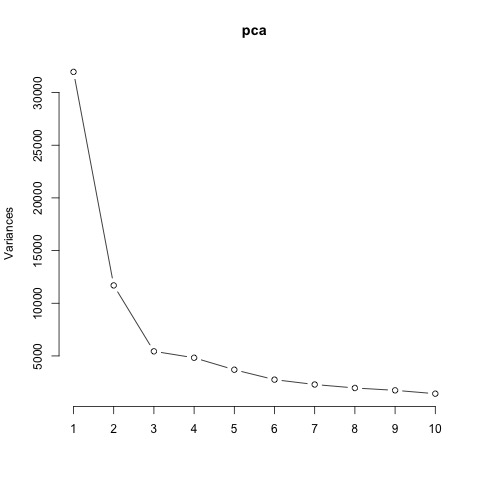
\includegraphics{screePlot}}
\captionof{figure}{Scree plot of the proportion of variance explained by each principal component for the DNase assay. The broken stick method selects 3 principal components, because the eigenvalue of the 4th component is not larger than the value given by the broken-stick distribution.}
\label{fig:figure2}
\end{figure}

\section{Clustering}

Subsequent to data normalization and principal component selection, an exploratory visualization of the transformed data was conducted to determine how best to proceed (Figure~\ref{fig:figure3}). This visualization revealed that although some tissue groups were tightly clustered, many of the points on the plot were not well clustered, or would intermingle with points from a different tissue group. 

\begin{figure}[tp]
\centering
\begin{minipage}{.5\textwidth}
	\centering
	\scalebox{1.10}{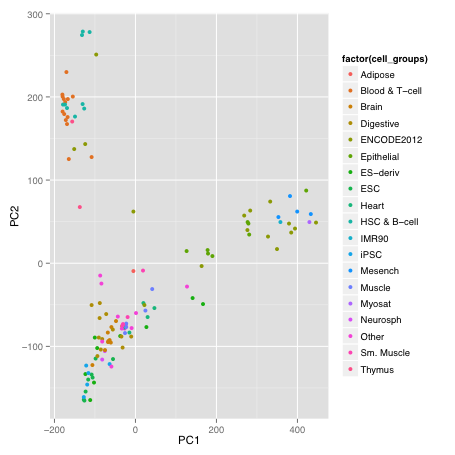
\includegraphics{scatternonormal}}
\end{minipage}%
\begin{minipage}{.5\textwidth}
	\centering
	\scalebox{1.10}{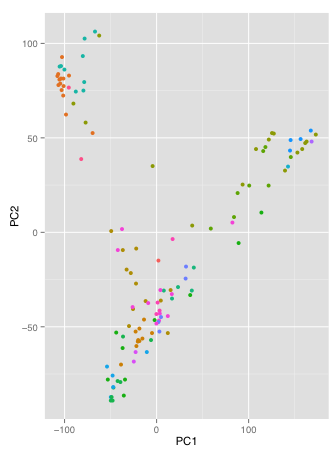
\includegraphics{scatternormal}}	
\end{minipage}	
\captionof{figure}{Scatter plot of the first two principal components of all 127 samples for DNase (a) prior to normalization and (b) after normalization. The tissue groups that each sample belongs to are denoted by color as indicated by the legend. .}
\label{fig:figure3}
\end{figure}

Our initial schema was to leverage a k-means approach to identify clusters within the data (in the number of PC dimensions as specified in Table~\ref{table:tab1}). This approach was based on the hypothesis that the variance from certain epigenetic modifications would allow classification of different tissues groups in the form of clusters (\citealp{Hein09}). To facilitate this procedure, the originally furnished dataset was subset to eliminate particular tissue groups that made the task less feasible. The {\it ENCODE2012} and {\it Other } tissue groups had representative cell types across multiple tissue types. These samples would be difficult to reclassify under the appropriate tissue group, and not all fit directly into the already established subcategories. Thus, the samples that comprised these two tissue groups were removed from the collection of data. Although this solution made the data more manageable, further reduction was required.  The objective function of k-means (Equation~\ref{eq:1}) has the intrinsic property of giving more weight to larger clusters; this property can be seen in Figure~\ref{fig:figure4}. To correct for this cluster size bias, smaller tissue groups, those with less than 5 samples per group, were also removed (mesench, neurosph, thymus, and sm. muscle). 

\begin{equation} \label {eq:1}
J = \Sigma^{k}_{j=1} \Sigma^{n}_{i=1} \abs{\abs{x^{(j)}_{i} - c_{j}}}
\end{equation}

\begin{figure}[tp]
\centering
\scalebox{.45}{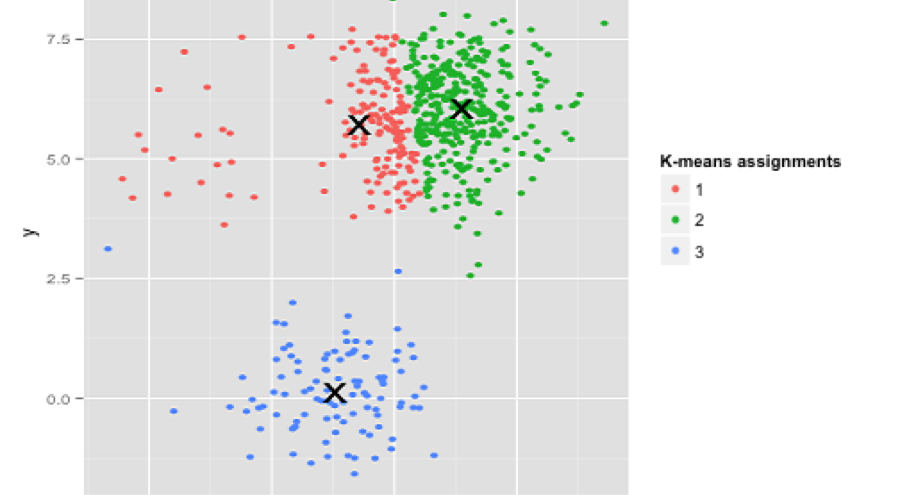
\includegraphics{kmeansex}}
\captionof{figure}{Clusters of size 20, 100, and 500 were generated from a multivariate Gaussian Distribution. K-means does not accurately assign the clusters as can be observed by individual inspection. This clustering algorithm assigns points that should be in cluster 2 into cluster 1 due the weight given to larger clusters.}
\label{fig:figure4}
\end{figure}

This final subset of the data resulted in a dataset comprised of 85 samples that represented 10 tissue groups and can be seen in Figure~\ref{fig:figure5}.

\begin{figure}[tp]
\centering
\scalebox{.45}{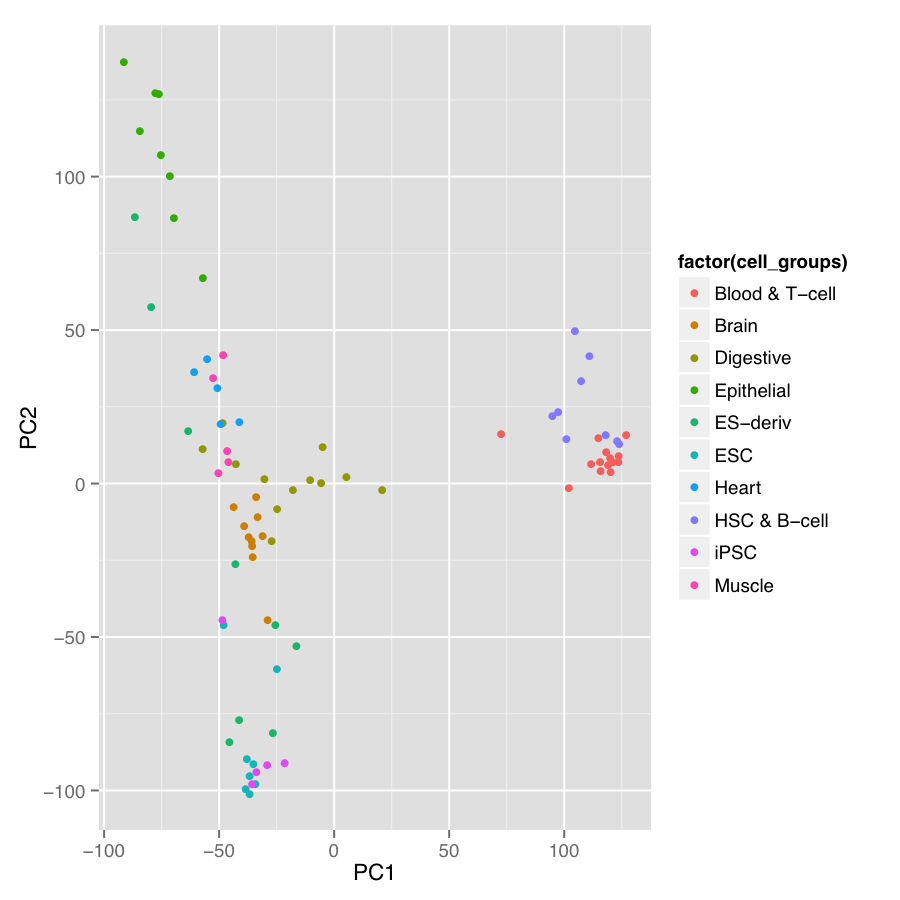
\includegraphics{kmeansfinal}}
\captionof{figure}{Scatter plot of the first two principal components of the 85 subset samples for DNase.}
\label{fig:figure5}
\end{figure}

It is clear that the data in Figure~\ref{fig:figure5} visibly falls into more defined clusters and is much more manageable to work with.

K-means clustering was implemented with the R stats package (\citealp{Rpkg}) which utilizes the algorithm from \citealp{Hart79}. The clustering was implemented on a variable number of principal components according to each epigenetic modification. Our objective was to recover the tissue types of each sample in the clusters with near 100\% purity. To achieve this, the number of clusters for k-means to ascertain was set to 10 (one cluster per tissue group). 
Visualizing the result of the k means clustering in 2 dimensions (especially when the clustering was done in more dimensions) would not be the best practice. To visually present the efficacy of our clustering methodology, heatmaps were constructed as seen in Figure~\ref{fig:figure6}a which have the tissue groups as columns and the clusters as rows. The heatmap indicates what percentage of each cluster an individual cell type represented (black being 0\%, orange being 50\%, and red being 100\%)

\begin{figure}[tp]
\centering
\begin{minipage}{.33\textwidth}
	\centering
	\scalebox{.45}{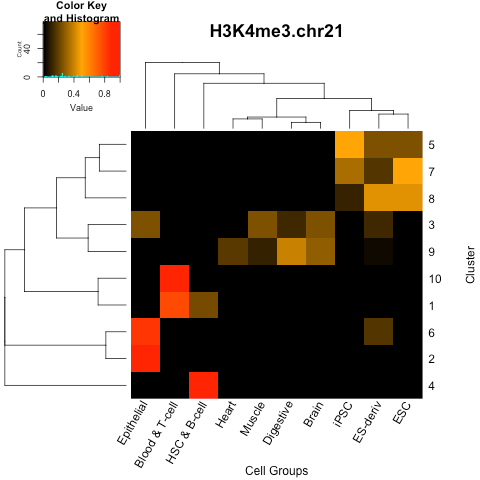
\includegraphics{heatmap1}}
\end{minipage}%
\begin{minipage}{.33\textwidth}
	\centering
	\scalebox{.45}{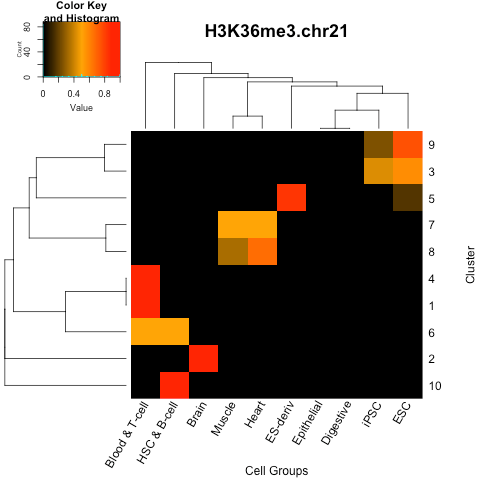
\includegraphics{heatmap2}}
\end{minipage}%
\begin{minipage}{.33\textwidth}
	\centering
	\scalebox{.45}{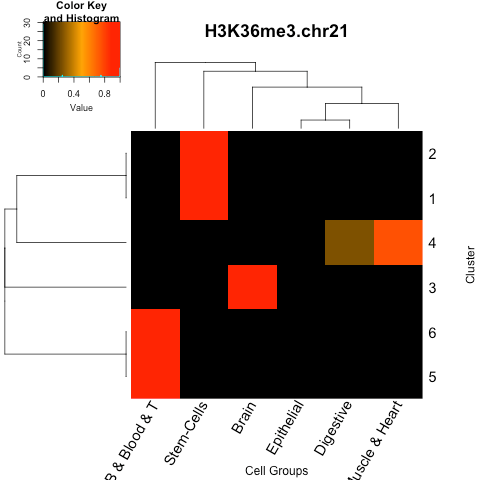
\includegraphics{heatmap3}}
\end{minipage}%
\captionof{figure}{Heatmap of clustering for H3K4me3 (a) k-means clustering, (b) tight clustering, (c) merged tight clustering. The columns represent the different tissue groups and the rows represent the different clusters. The heatmap indicates what percentage of each cluster an individual tissue group comprised (black being 0\%, orange being 50\%, and red being 100\%)}
\label{fig:figure6}
\end{figure}

\begin{equation} \label{eq:2}
\bf{P} = \frac{\bf{TP}}{\bf{TP} + \bf{FP}} \qquad
 \bf{R} = \frac{\bf{TP}}{\bf{TP} + \bf{FN}} \qquad
 \bf{F}_\beta = \frac{(\beta^2 + 1)\bf{PR}}{\beta^2\bf{P} + \bf{R}}
\end{equation}
\\

Using this methodology, it became apparent that the tissue types {\it Blood} \& {\it T-cells}, {\it HSC} \& {\it B-cells}, and {\it digestive cells} were most consistently representative of an entire cluster (these cell types were the easiest to cluster across epigenetic modifications). Additionally, {\it iPSC}, {\it ES-deriv}, and {\it ESC} tissue types appeared in the same clusters across multiple epigenetic modifications, indicating a difficulty in characterizing these tissue groups using epigenetic modifications. A similar joint cluster effect was also identified in {\it heart} and {\it muscle} tissue groups. 

To evaluate the effectiveness of this clustering methodology, a variation of the F-score ($F_{\beta}$) was used (\citealp{Man08}). The F-score uses precision and recall which can be employed to rate the effectiveness of a clustering methodology. This particular variation of the F-score includes a $\beta$ term which weights the F-score towards recall; it penalizes false negatives more strongly than false positives (Equation~\ref{eq:2}). The $F_{\beta}$ score is used to evaluate the effectiveness of our clustering methodologies. It is a weighted ratio of the precision and recall of the clustering classification.

\begin{table}[t]
	\tbl{F-Scores and Purity Scores}{
	\resizebox{\textwidth}{!}{
		\begin{tabular}{|l|l|l|l|l|l|l|l|l|l|}
			\hline
			& DNase    & H3K27ac  & H3K27me3 & H3K36me3 & H3K4me1  & H3K4me3  & H3K9ac   & H3K9me3  & RNAseq   \\ \hline
			F-Scores & 0.59444  & 0.62777  & 0. 39444 & 0. 58055 & 0. 51666 & 0. 54166 & 0. 4555  & 0. 35555 & 0. 5083  \\ \hline
			Purity   & 0.576470 & 0.705882 & 0.682352 & 0.705882 & 0.752941 & 0.741176 & 0.682352 & 0.658823 & 0.682352 \\ \hline
		\end{tabular}}}
		\begin{tabnote}
			Table~\ref{table:tab2} - F-scores and purity scores for the k-means clustering of 85 samples comprising 10 tissue groups across different epigenetic modifications
		\end{tabnote}
		\label{table:tab2}
\end{table}

These F-scores do not vary much with regards to epigenetic modification, however, using this methodology, the F-score suggests that H3K27ac is the most cell type specific epigenetic modification.

Purity scores (Equation~\ref{eq:3}) are also included for comparison in the k-means clustering analysis due to their propensity to better explain clustering success in methods employed later in the manuscript. They are used to evaluate the composition of each cluster. The purity is computed by summing the most prevalent tissue group in each cluster and dividing that sum by the total samples in all the clusters (\citealp{Man08}). It is interesting to note that H3K27ac, which had the highest F-score, did not have the highest (or second highest) purity score.

\begin{equation} \label{eq:3}
purity(\Omega,\mathbb{C}) = \frac{1}{N}\sum_{k}max_{j}\abs{\omega_k \cap c_j }
\end{equation}
\\

A common issue with k-means that could explain the low F-scores is the requirement that every data point be a member of a cluster. Here, we argue that a more reasonable approach for this type of data is a tight clustering approach that only identifies points that are tightly clustered together and does not require every data point to be a part of a cluster (\citealp{tClust}).  

Using this tight clustering methodology, we obtained the top 10 tight clusters for each epigenetic modification, and generated heatmaps Figure~\ref{fig:figure6}b using a similar method to that employed in the k-means pipeline. 

The heatmaps generated using tight clustering consistently have a greater number of “red” features than the k-means clustering yielded, however, the tight clustering approach resulted in many tissue types as members of more than one cluster (there is trade off in the “tightness” parameter with how similar the objects in the cluster are vs. how many elements are in the cluster). These features are well illustrated by the F-scores and purity scores for the tight clustering technique. The F-scores are in general lower than the corresponding F-scores for the k-means clustering due to tight clustering yielding two (or three) clusters comprised of a single tissue type (i.e. {\it Blood \& T-cell} in Figure~\ref{fig:figure6}b). Although the purity of these clusters is very high (as reflected in Table~\ref{table:tab3}) the F-scores are low when a tissue type is split into multiple clusters due to a high rate of false negatives.

\begin{table}[t]
	\tbl{F-Scores and Purity Scores}{
	\resizebox{\textwidth}{!}{
		\begin{tabular}{|l|l|l|l|l|l|l|l|l|l|}
			\hline
			& DNase     & H3K27ac   & H3K27me3  & H3K36me3  & H3K4me1   & H3K4me3 & H3K9ac   & H3K9me3   & RNAseq   \\ \hline
			F-Scores & 0.2845528 & 0.4933333 & 0.1792452 & 0.3653846 & 0.4631578 & 0.5125  & 0.625    & 0.3557692 & 0.416    \\ \hline
			Purity   & 0.707317  & 0.769230  & 0.512195  & 0.789473  & 0.868421  & 0.7     & 0.880952 & 0.75      & 0.682352 \\ \hline
		\end{tabular}}}
		\begin{tabnote}
			Table~\ref{table:tab3} - F-scores and purity scores for the tight clustering of 85 samples comprising 10 tissue groups across different epigenetic modifications
		\end{tabnote}
		\label{table:tab3}
\end{table}

Although many of these F-scores were worse than those resulting from k-means, we noticed that a number of the tissue groups clustered together throughout the different epigenetic markers. These tissue types were merged into larger, representative tissue groups and tight clustering was performed anew. Specifically, {\it Blood \& T-cells} and {\it HSC \& B-cells} were merged into one group; {\it iPSC, ES-deriv,} and {\it ESC} were merged into another group; {\it heart} and {\it muscle} were merged into a final group. This merging resulted in six total tissue groups (three merged groups of seven total tissue groups and the three remaining unmerged tissue groups). The pipeline was rerun on this new merged dataset and resulted in one final heatmap (~\ref{fig:figure6}c) with corresponding F-scores and purity scores (Table~\ref{table:tab4}).

\begin{table}[t]
	\tbl{F-Scores and Purity Scores}{
	\resizebox{\textwidth}{!}{
		\begin{tabular}{|l|l|l|l|l|l|l|l|l|l|}
			\hline
			& DNase    & H3K27ac  & H3K27me3  & H3K36me3  & H3K4me1   & H3K4me3   & H3K9ac   & H3K9me3   & RNAseq   \\ \hline
			F-Score & 0.52380  & 0.697478 & 0.4895104 & 0.5545454 & 0.5726495 & 0.4171779 & 0.713178 & 0.3972602 & 0.603351 \\ \hline
			Purity  & 0.769230 & 1        & 0.777777  & 1         & 1         & 0.8181818 & 1        & 1         & 1        \\ \hline
		\end{tabular}}}
		\begin{tabnote}
			Table~\ref{table:tab4} - F-scores and purity scores for the merged tight clustering of 85 samples comprising 6 merged tissue groups across different epigenetic modifications
		\end{tabnote}
		\label{table:tab4}
\end{table}

Although these F-scores are considerably better than those generated by the unmerged tight clustering methodology, they still tend to suffer from the same false negative drawback. However, using this methodology, it appears that H3K27ac and H3K9ac are the most cell-type specific epigenetic modifications. This is further confirmed by a purity score of 1 for the tissue group clusters that resulted from these epigenetic modifications.

\section{Variance Analysis}
Since similar cell types seemed to cluster together in our analysis, we then sought to understand whether certain genomic regions are more important than others in explaining the similarity of the cell-types, which could point to these regions having an important biological function. However, the weight of each region on the important principal components was at most 0.01 for any genomic region and epigenomic mark. 
Even though the differences in the loadings of the principal components were small, this could be caused by the fact that the data is binned in regions of 500 base pairs which might be either too large or too small to have a significant contribution. Since higher resolution data was not immediately available, we binned the hundred most important regions into segments of 5kb to see whether certain 5kb regions contain more of the important loadings than others. Since certain 5kb regions seemed to be more important than others (Figure ~\ref{fig:figure7}), we investigated whether the regions where the top loadings clustered had a biological function. A preliminary analysis using the UCSC Genome Browser (\cite{UCSC}), showed that these fell predominantly in non-coding regions. However, since previous work points to a connection between histone modifications and enhancer sites, which can be far from the coding region they regulate, we overlapped these regions with the enhancer sites predicted by ChromHMM (\cite{Ernst12}) in 9 different cell types. Even though the ChromHMM tracks are imputed, they provide the most comprehensive and widely accepted annotation of human enhancer sites across cell-types. Although some regions overlapped with strong or weak enhancer sites, this overlap was not consistent enough for any further claims to be made. There were also no regions that consistently appeared over multiple epigenetic marks. Therefore, it seems that the cell type specificity of epigenetic marks is not based on one particular region in the genome, but rather in the way they alter the chromatin at chromosome level.

\begin{figure}[tp]
\centering
\scalebox{.45}{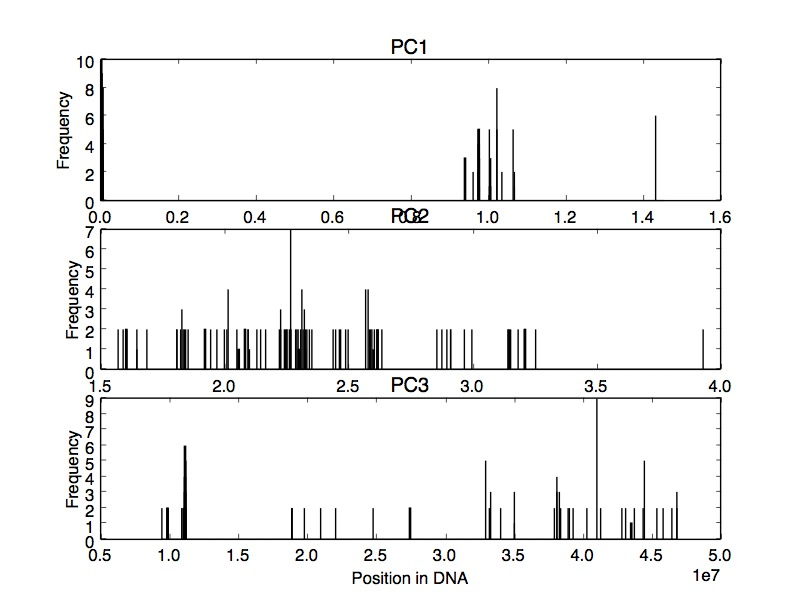
\includegraphics{regions}}
\captionof{figure}{Histogram of the distribution of 500 base pair bins across the genome, binned together into regions of 5kb for the H3K4me3 histone modification. Certain bins show a higher frequency of important regions than others. See Suplementary Material for this figure in all epigenetic marks.}
\label{fig:figure7}
\end{figure}

\begin{thebibliography}{}
\bibitem[Ernst and Kellis, 2015]{Ernst15} Jason Ernst and Manolis Kellis. (2015) Large-scale imputation of epigenomic datasets for systematic annotation of diverse human tissues, {\it Nature Biotechnology}, {\bf 33}, 364-376.
\bibitem[Cangelosi and Goriely, 2007]{Cang07} Richard Cangelosi and Alain Goriely. (2007) Component retention in principal component analysis with application to cDNA microarray data, {\it Biology Direct}, {\bf 2}, 2.
\bibitem[Heintzman {\it et~al}.,  2009]{Hein09} Heintzman N. D., {\it et~al}. (2009) Histone modifications at human enhancers reflect global cell-type-specific gene expression, {\it Nature}, {\bf 459}, 108-112.
\bibitem[Hartigan and Wong, 1979]{Hart79} J. A. Hartigan and M. A. Wong. (1979) Algorithm AS 136: A K-Means Clustering Algorithm, {\it Journal of the Royal Statistical Society. Series C (Applied Statistics)}, {\bf 28}, 100-108.
\bibitem[RCoreTeam, 2015]{Rpkg} R Core Team (2015). R: A language and environment for statistical computing. R Foundation for Statistical Computing, Vienna, Austria. URL http://www.R-project.org/
\bibitem[Manning {\it et~al}.,  2008]{Man08} Christopher D. Manning, Prabhakar Raghavan and Hinrich Schütze, Introduction to Information Retrieval, Cambridge University Press. 2008, 357-359
\bibitem[Tseng and Wong, 2012]{tClust} George C. Tseng and Wing H. Wong (2012). tightClust: Tight Clustering. R package version 1.0. http://CRAN.R-project.org/package=tightClust
\bibitem[Rosenbloom {\it et~al}., 2015]{UCSC} Rosenbloom KR, {\it et~al}. (2015) The UCSC Genome Browser database: 2015 update, {\it Nucleic Acids Res.}, {\bf 43}, 670-81.
\bibitem[Ernst and Kellis, 2012]{Ernst12} Jason Ernst and Manolis Kellis. (2012) ChromHMM: automating chromatin-state discovery and characterization, {\it Nature Methods}, {\bf 9}, 215-216.
\end{thebibliography}{}

\end{document}
% End of v2-acmlarge-sample.tex (March 2012) - Gerry Murray, ACM
